\section*{Parte (a)}

\subsection*{(a)}
Explique o que essa visualização representa e interprete os resultados obtidos.

\vspace{0.5em}
\noindent A visualização da figura "attention.html" representa a matriz que correlaciona cada uma das 32 primeiras amostras do conjunto de teste às outras amostras. O valor de cada aresta é dado pelo produto interno entre as vetorizações TF-IDF de cada par de notícias, ou seja, a similaridade entre dois textos dadas suas palavras ponderadas pelo inverso da frequência.

\vspace{0.5em}
\noindent O código que gera esta visualização:

\begin{lstlisting}[language=Python]
seq = X_test[:32,:]
b = seq.toarray()
att = b@b.T
att = att.reshape(1,1,32,32)
att = torch.tensor(att)
counts = [0,0,0,0]
tokens = []
for i in y_test[:32]:
    token = target_names[i] + ' ' + str(counts[i])
    tokens.append(token)
    counts[i]+=1
head_view((att,), tokens)
\end{lstlisting}

\noindent A matriz de atenção $att$ é calculada como $att = b \cdot b^T$, onde $b$ são as representações TF-IDF das 32 primeiras amostras.
Esta operação produz uma matriz 32x32 onde cada entrada $(i,j)$ representa a similaridade cosseno entre as amostras $i$ e $j$.

\begin{figure}[h]
    \centering
    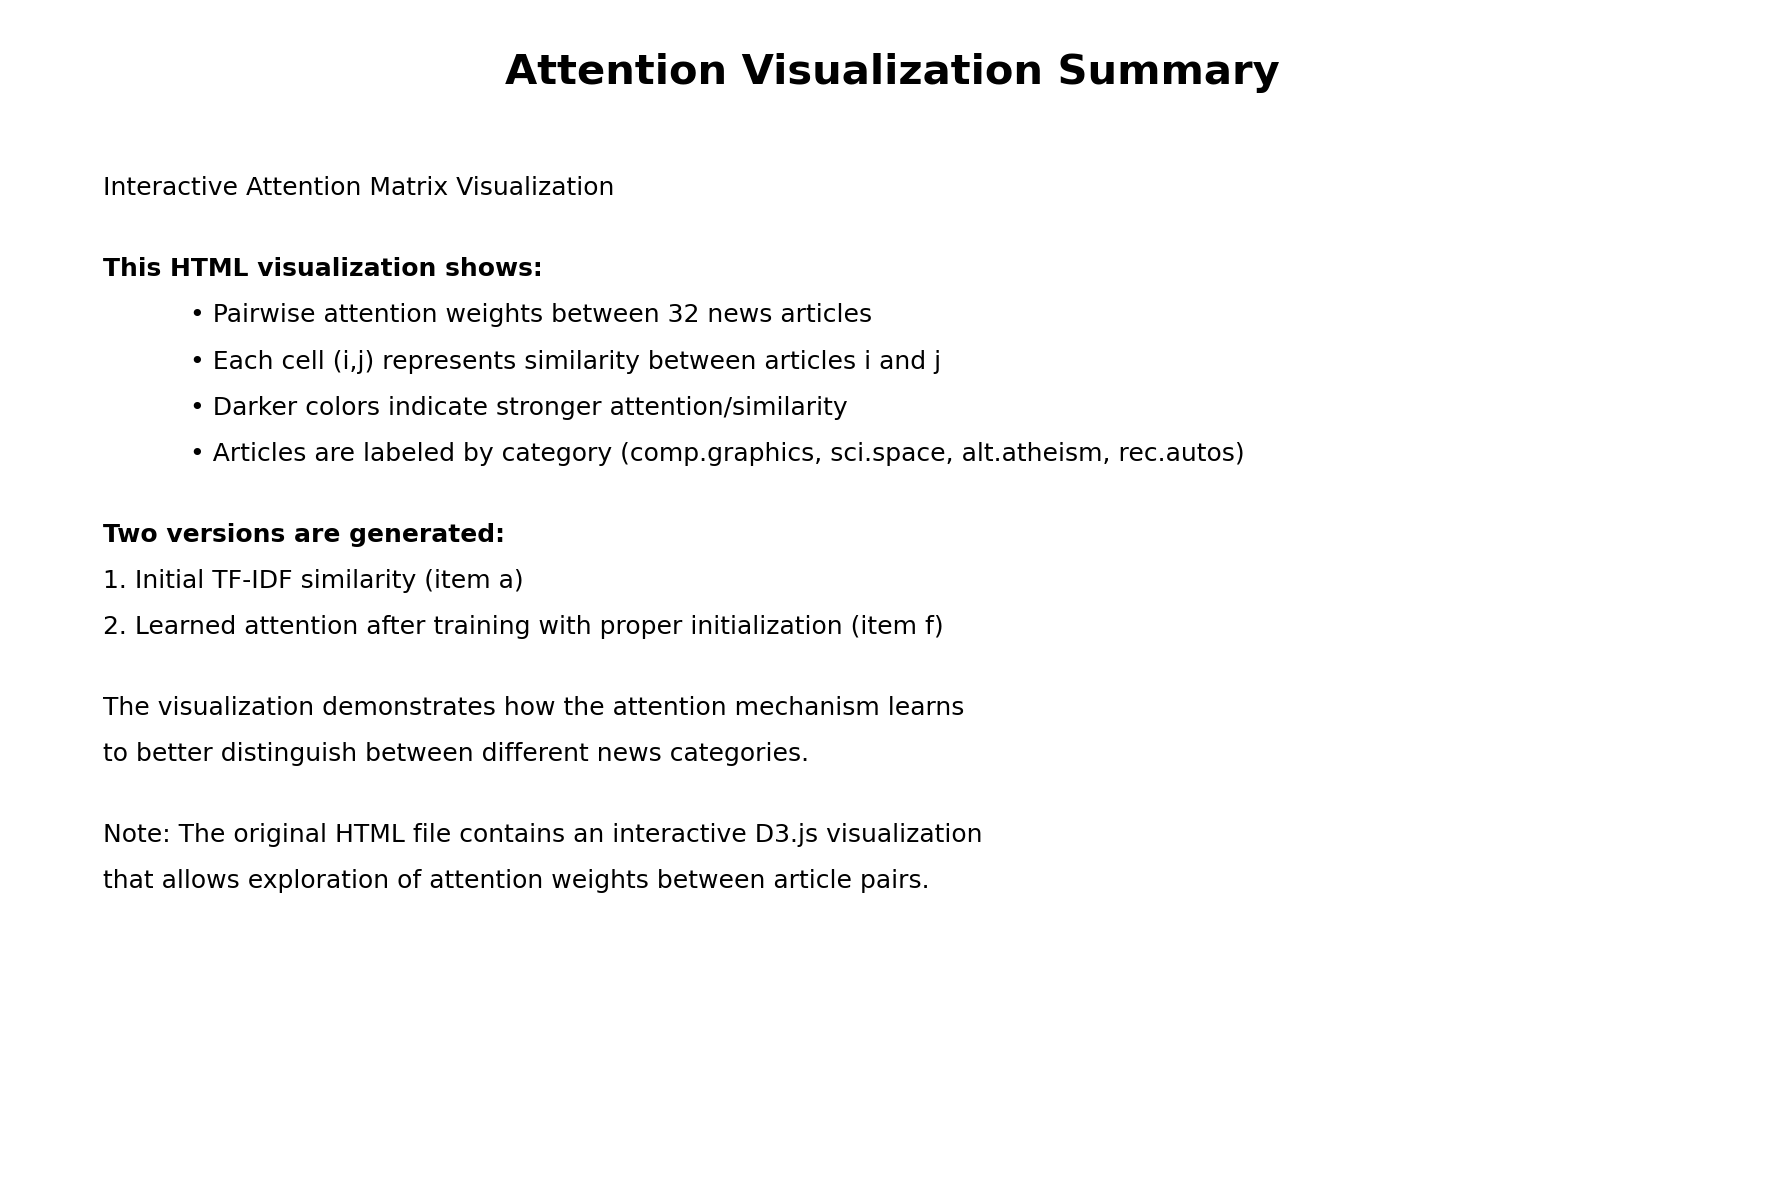
\includegraphics[width=0.8\textwidth]{../figures/4/attention_visualization_description.png}
    \caption{Descrição da visualização de atenção TF-IDF}
    \label{fig:attention_description}
\end{figure}

\section*{Parte (b)}

\subsection*{(b-i)}
Sejam $u, v \in \mathbb{R}^d$, $P_u$ a projeção ortogonal sobre o espaço gerado por $u$. Mostre que $P_u(v) = \frac{\langle u, v \rangle}{\|u\|^2} u$.

\vspace{0.5em}
\noindent A projeção do vetor $v$ em $u$ tem duas componentes: direção e magnitude. A direção é dada pelo vetor de norma unitária na direção de $u$:
\begin{equation*}
    \hat{u} = \frac{u}{\|u\|}
\end{equation*}

\noindent A magnitude é dada pela componente de $v$, $v_u$, tal que $v - v_u = v_{\perp u}$ e $v_{\perp u}$ é ortogonal a $u$. $v_u$ é também a projeção escalar de $v$ em $u$, cuja definição é:
\begin{equation*}
    v_u = v \cdot \hat{u} = \frac{v \cdot u}{\|u\|}
\end{equation*}

\noindent Assim:
\begin{align*}
    P_u(v) & = v_u \cdot \hat{u}                             \\
           & = \frac{v \cdot u}{\|u\|} \cdot \frac{u}{\|u\|} \\
           & = \frac{\langle v, u \rangle}{\|u\|^2} \cdot u
\end{align*}

\subsection*{(b-ii)}
Considere a definição de cosseno entre dois vetores $\cos(u, v) := \frac{\langle u, v \rangle}{\|u\|\|v\|}$. Use a fórmula do item (b-i) para relacionar essa definição de cosseno com o cosseno de um ângulo (construa um triângulo retângulo com $v$ e $P_u(v)$).

\vspace{0.5em}
\noindent Partindo da definição:
\begin{equation*}
    \cos(u, v) := \frac{\langle u, v \rangle}{\|u\|\|v\|}
\end{equation*}

\noindent Substituindo a relação encontrada em (b-i):
\begin{align*}
    \cos(u, v) & = P_u(v) \cdot \frac{\|u\|}{\|v\|} \cdot u          \\
               & = \frac{P_u(v)}{\hat{u}\|v\|}                       \\
               & = \frac{\|P_u(v)\|\hat{u}}{\|v\|\hat{u}}            \\
               & = \frac{\|P_u(v)\|}{\|v\|}                          \\
               & = \frac{\text{Cateto Adjacente}}{\text{Hipotenusa}}
\end{align*}

\subsection*{(b-iii)}
Mostre que, se $u_1, v_1, u_2, v_2 \in \mathbb{R}^d$ com $\|u_1\| = \|v_1\| = \|u_2\| = \|v_2\| = 1$, então $\cos(u_1, v_1) \geq \cos(u_2, v_2) \iff \|u_1 - v_1\| \leq \|u_2 - v_2\|$. Argumente que $\cos$ pode ser usado como uma medida de similaridade quando os vetores em consideração têm norma 1.

\vspace{0.5em}
\noindent Assumindo:
\begin{align*}
    \cos(u_1, v_1)           & \geq \cos(u_2, v_2)           \\
    \langle u_1, v_1 \rangle & \geq \langle u_2, v_2 \rangle \\
    P_{u_1}(v_1)             & \geq P_{u_2}(v_2)
\end{align*}

\noindent Calculando a norma da diferença $\|u_1 - v_1\|$:
\begin{align*}
    \|u_1 - v_1\| & = \left[ (\|u_1\| + \|-v_1\|)^2 - 2\|P_{u_1}(v_1)\| \right]^{\frac{1}{2}} \\
                  & = [1 + 1 - 2\|P_{u_1}(v_1)\|]^{\frac{1}{2}}                               \\
                  & = [2 - 2\|P_{u_1}(v_1)\|]^{\frac{1}{2}}
\end{align*}

\noindent Analogamente para $\|u_2 - v_2\|$:
\begin{equation*}
    \|u_2 - v_2\| = [2 - 2\|P_{u_2}(v_2)\|]^{\frac{1}{2}}
\end{equation*}

\noindent Portanto, se $\|P_{u_1}(v_1)\| \geq \|P_{u_2}(v_2)\|$, então $\|u_1 - v_1\| \leq \|u_2 - v_2\|$, já que $[1 - \|P_{u_1}(v_1)\|] \leq [1 - \|P_{u_2}(v_2)\|]$. O sentido oposto da prova é feito de maneira análoga.

\noindent Conclui-se que o cosseno pode ser usado como uma métrica de similaridade equivalente à norma da diferença (distância), com escala variando de $1$ (vetores com mesma direção e sentido) a $-1$ (vetores com sentidos opostos), sendo $0$ para vetores ortogonais.

\subsection*{(b-iv)}
Em vista do item anterior, aponte diferenças entre a noção de similaridade capturada por $\|u - v\|$ e $\cos(u, v)$. Em que casos seria mais vantajoso usar cada uma dessas noções de similaridade?

\vspace{0.5em}
\noindent A métrica da norma da diferença tem seus valores proporcionais à magnitude dos vetores avaliados. Enquanto isso, a métrica do cosseno pressupõe vetores unitários e é agnóstica à magnitude.

\noindent Assim, em um caso em que apenas a direção importa, o cosseno é preferível. Em casos em que a magnitude também é relevante, a métrica da norma é preferível ao cosseno.

\section*{Parte (c)}

\subsection*{(c)}
Note que a rede não está aprendendo. Explique qual é o problema e exponha evidências de que ele realmente está acontecendo.

\vspace{0.5em}
\noindent A inicialização incorreta da matriz de pesos é a causa do não aprendizado da rede. Como não normalizamos os pesos, sua variância era grande o suficiente para gerar valores com alta magnitude que, ao passar pelo softmax, resulta em valores próximos a 1 com gradientes próximos a 0.

\vspace{0.5em}
\noindent O problema pode ser observado através das evidências experimentais:

\begin{enumerate}
    \item \textbf{Perda constante}: O gráfico da função perda mostra que ela permanece praticamente constante ao longo das épocas, indicando ausência de aprendizado.

    \item \textbf{Gradientes próximos a zero}: Os histogramas dos gradientes das matrizes $A_K$ e $A_Q$ mostram que a maioria dos gradientes está concentrada em torno de zero, evidenciando o problema do gradiente que desaparece.

    \item \textbf{Saída do softmax saturada}: O histograma da saída do softmax mostra valores próximos a 1, indicando saturação da função.
\end{enumerate}

\begin{figure}[h]
    \centering
    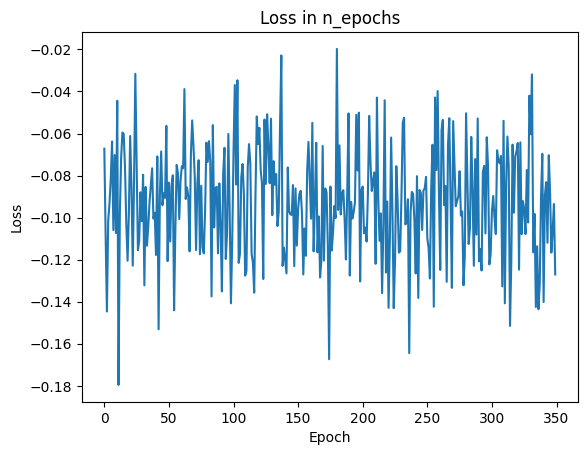
\includegraphics[width=0.7\textwidth]{../figures/4/loss_no_init_fix.png}
    \caption{Função perda sem inicialização adequada - sem aprendizado}
    \label{fig:loss_no_init}
\end{figure}

\begin{figure}[h]
    \centering
    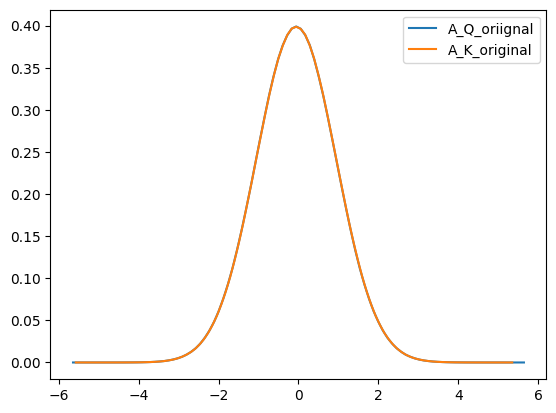
\includegraphics[width=0.7\textwidth]{../figures/4/weight_distributions_no_init_fix.png}
    \caption{Distribui\c{c}\~{o}es dos pesos iniciais $A_K$ e $A_Q$}
    \label{fig:weights_no_init}
\end{figure}

\begin{figure}[h]
    \centering
    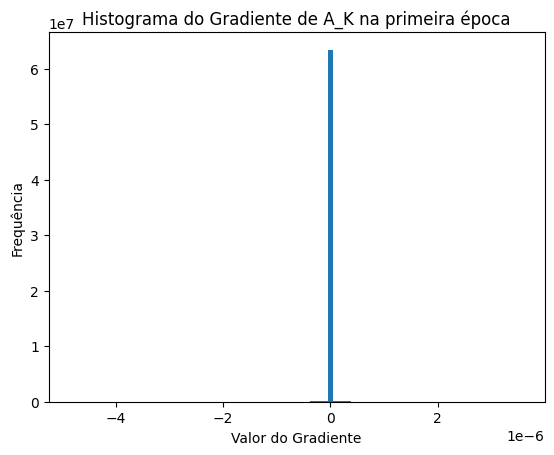
\includegraphics[width=0.45\textwidth]{../figures/4/gradient_histogram_A_K_no_init_fix.png}
    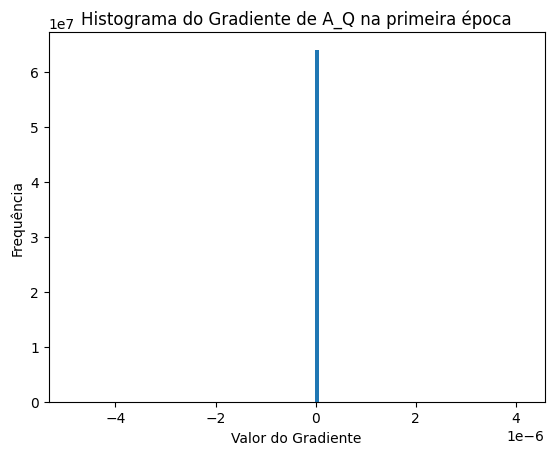
\includegraphics[width=0.45\textwidth]{../figures/4/gradient_histogram_A_Q_no_init_fix.png}
    \caption{Histogramas dos gradientes de $A_K$ e $A_Q$ na primeira \'{e}poca (sem inicializa\c{c}\~{a}o adequada)}
    \label{fig:gradients_no_init}
\end{figure}

\begin{figure}[h]
    \centering
    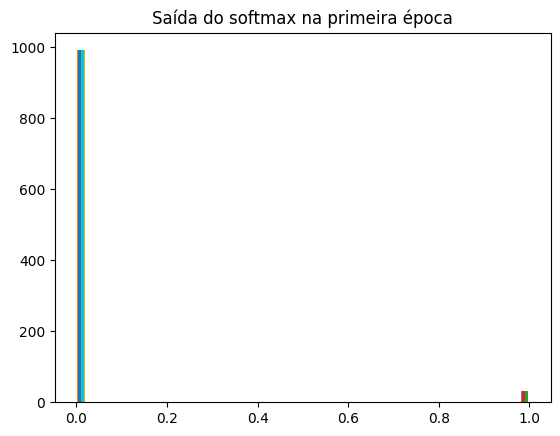
\includegraphics[width=0.7\textwidth]{../figures/4/softmax_output_no_init_fix.png}
    \caption{Sa\'{i}da do softmax na primeira \'{e}poca (sem inicializa\c{c}\~{a}o adequada)}
    \label{fig:softmax_no_init}
\end{figure}

\vspace{0.5em}
\noindent O c\'{o}digo que demonstra esse problema:

\begin{lstlisting}[language=Python]
# Inicialização sem normalização adequada
A_K = torch.randn((D,D)).cuda()  # SEM *init_scale(D)
A_Q = torch.randn((D,D)).cuda()  # SEM *init_scale(D)

# Loop de treinamento
for epoch in range(n_epochs):
    # ... treinamento ...
    att = softmax((K.T@Q)/(D**(1/2)))
    loss = -cos(att,truth).mean()
    loss.backward()
\end{lstlisting}

\section*{Parte (d)}

\subsection*{(d)}
Corrija o problema identificado no item anterior e demonstre que a rede agora consegue aprender.

\vspace{0.5em}
\noindent De fato, adicionar um termo na inicialização dos parâmetros permitiu o aprendizado e subsequente redução da função perda. Isso ocorre pois o valor pelo qual multiplicamos os pesos iniciais é $(2/D)^{1/2}$, sendo $D$ o tamanho da camada. Isso reduz a variância dos parâmetros e evita que valores muito grandes sejam passados ao softmax e tenham seu gradiente próximo a zero.

\vspace{0.5em}
\noindent A correção implementada:

\begin{lstlisting}[language=Python]
def init_scale(fan_in):
    return (2/fan_in)**0.5

# Inicialização com normalização adequada
A_K = torch.randn((D,D)).cuda() * init_scale(D)  # COM *init_scale(D)
A_Q = torch.randn((D,D)).cuda() * init_scale(D)  # COM *init_scale(D)
\end{lstlisting}

\vspace{0.5em}
\noindent As evidências do aprendizado bem-sucedido incluem:

\begin{enumerate}
    \item \textbf{Redução da perda}: O gráfico da função perda agora mostra uma tendência decrescente clara ao longo das épocas.

    \item \textbf{Gradientes não-zero}: Os histogramas dos gradientes mostram distribuições mais amplas, indicando gradientes efetivos para o aprendizado.

    \item \textbf{Distribuição melhorada do softmax}: A saída do softmax apresenta uma distribuição mais balanceada, não saturada.
\end{enumerate}

\begin{figure}[h]
    \centering
    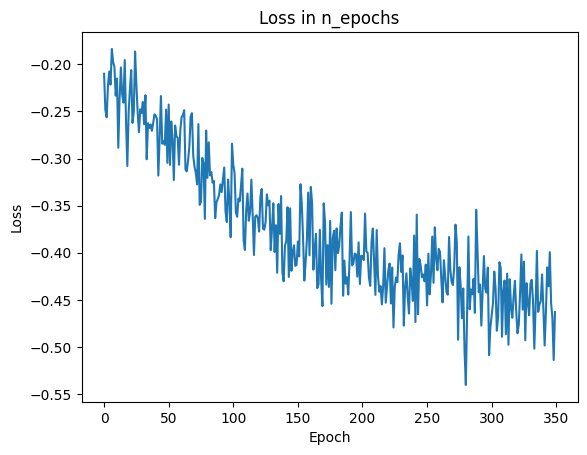
\includegraphics[width=0.7\textwidth]{../figures/4/loss_with_init_fix.png}
    \caption{Fun\c{c}\~{a}o perda com inicializa\c{c}\~{a}o adequada - aprendizado bem-sucedido}
    \label{fig:loss_with_init}
\end{figure}

\begin{figure}[h]
    \centering
    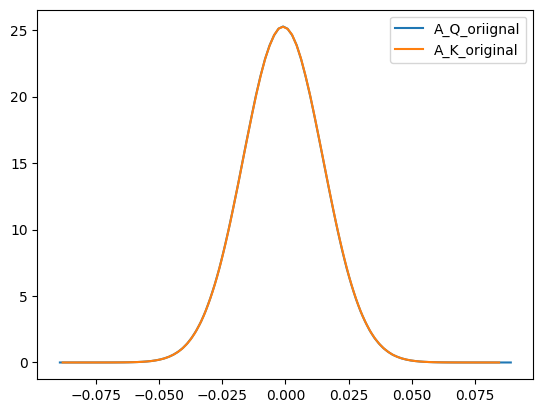
\includegraphics[width=0.7\textwidth]{../figures/4/weight_distributions_with_init_fix.png}
    \caption{Distribui\c{c}\~{o}es dos pesos iniciais $A_K$ e $A_Q$ com inicializa\c{c}\~{a}o adequada}
    \label{fig:weights_with_init}
\end{figure}

\begin{figure}[h]
    \centering
    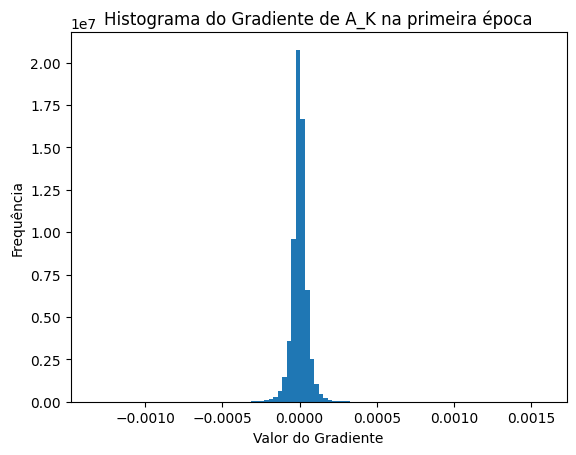
\includegraphics[width=0.45\textwidth]{../figures/4/gradient_histogram_A_K_with_init_fix.png}
    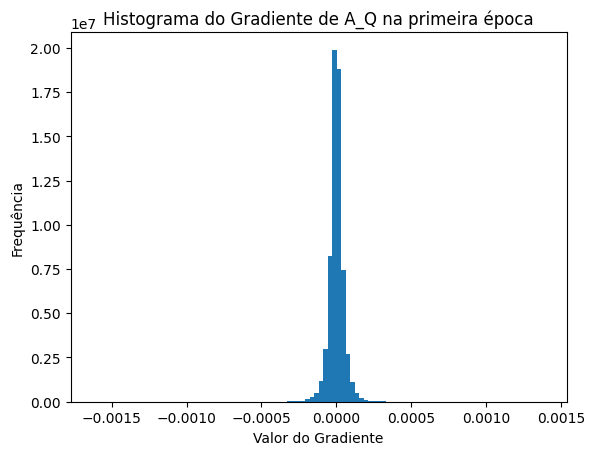
\includegraphics[width=0.45\textwidth]{../figures/4/gradient_histogram_A_Q_with_init_fix.png}
    \caption{Histogramas dos gradientes de $A_K$ e $A_Q$ na primeira \'{e}poca (com inicializa\c{c}\~{a}o adequada)}
    \label{fig:gradients_with_init}
\end{figure}

\begin{figure}[h]
    \centering
    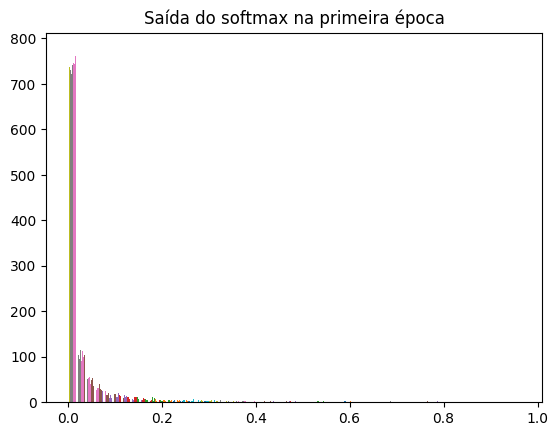
\includegraphics[width=0.7\textwidth]{../figures/4/softmax_output_with_init_fix.png}
    \caption{Sa\'{i}da do softmax na primeira \'{e}poca (com inicializa\c{c}\~{a}o adequada)}
    \label{fig:softmax_with_init}
\end{figure}


\section*{Parte (e)}

\subsection*{(e-i)}
A camada de auto-atenção (self-attention) pode ser representada matematicamente como
\begin{equation*}
    \text{Sa}[X] = V[X] \cdot \text{Softmax} \left( \frac{K[X]^T Q[X]}{\sqrt{D}} \right)
\end{equation*}
Mostre que, se $K[X]$ e $Q[X]$ têm entradas gaussianas com média zero e variância $\sigma^2$, todas independentes entre si, cada entrada de $K[X]^T Q[X]$ tem variância $\sigma^4 D$. Use esse fato para argumentar a favor da divisão por $\sqrt{D}$.

\vspace{0.5em}
\noindent Seja $Z = K[X]^T Q[X] = \sum_{i=1}^D K_i[X]^T Q_i[X]$

\noindent Calculando a Esperança $\mathbb{E}(Z)$:
\begin{align*}
    \mathbb{E}(Z) & = \mathbb{E}(K[X]^T Q[X])                                                         \\
                  & = \mathbb{E}(K[X]^T) \cdot \mathbb{E}(Q[X]) \quad \text{(devido à independência)} \\
                  & = 0 \cdot 0 = 0
\end{align*}

\noindent Calculando a Variância $\mathbb{V}(Z)$:
\begin{align*}
    \mathbb{V}(Z) & = \mathbb{V}(K[X]^T Q[X])                                                 \\
                  & = \mathbb{E}\left([K[X]^T Q[X] - \mathbb{E}(K[X]^T Q[X])]^2\right)        \\
                  & = \mathbb{E}\left((K[X]^T Q[X])^2\right) - (\mathbb{E}(K[X]^T Q[X]))^2    \\
                  & = \mathbb{E}\left((K[X]^T)^2\right) \cdot \mathbb{E}\left((Q[X])^2\right)
\end{align*}

\noindent Como $\mathbb{V}(K[X]^T) = \mathbb{E}\left((K[X]^T)^2\right) - (\mathbb{E}[K[X]^T])^2$:
\begin{equation*}
    \mathbb{V}(K[X]^T) = \mathbb{E}\left((K[X]^T)^2\right)
\end{equation*}

\noindent Logo, $\mathbb{V}(Z) = \mathbb{V}(K[X]^T) \cdot \mathbb{V}(Q[X])$

\noindent A variância de cada termo na soma é $\sigma^2 \cdot \sigma^2 = \sigma^4$. Somando sobre as $D$ dimensões:
\begin{equation*}
    \mathbb{V}(Z)_{ij} = \sum_{i=1}^D \sigma^4 = D\sigma^4
\end{equation*}

\noindent Para normalizarmos e obtermos variância unitária, devemos dividir pela raiz da variância. Como $\sigma$ é comum a ambos os termos da divisão, apenas $\sqrt{D}$ aparece no denominador.

\subsection*{(e-ii)}
É necessário assumir que as entradas são gaussianas para chegar a essa conclusão? Caso contrário, é necessário que sejam identicamente distribuídas?

\vspace{0.5em}
\noindent Não foi necessário assumir distribuição gaussiana das variáveis, apenas independência e mesmos valores de média e variância. Os mesmos resultados seriam obtidos caso as variáveis não seguissem a mesma distribuição, mas mantivessem a independência e os valores de média e variância constantes.

\section*{Parte (f)}

\subsection*{(f)}
Usando o comando head\_view, visualize a similaridade par a par que a rede associa à sequência de notícias correspondente a X\_test[:32], y\_test[:32]. Compare com a visualização realizada no item (a) e interprete o resultado.

\vspace{0.5em}
\noindent O resultado do presente head\_view apresenta relações entre amostras da mesma classe mais fortes que o head\_view do item (a), indicando o impacto do treinamento na definição da similaridade.

\vspace{0.5em}
\noindent O código que gera a visualização após o treinamento:

\begin{lstlisting}[language=Python]
# Calculando a nova matriz de atenção com os pesos treinados
att = (A_K.cpu().detach().numpy()@b.T ).T @ (A_Q.cpu().detach().numpy()@b.T )
att = att.reshape(1,1,32,32)
att = torch.tensor(att)
head_view((att,), tokens)
\end{lstlisting}

\vspace{0.5em}
\noindent A comparação entre as visualizações mostra:

\begin{enumerate}
    \item \textbf{Visualização inicial (item a)}: Utiliza similaridade TF-IDF pura ($b \cdot b^T$), onde a similaridade é baseada apenas na sobreposição de termos ponderados.

    \item \textbf{Visualização após treinamento (item f)}: Utiliza as matrizes aprendidas $A_K$ e $A_Q$, calculando $(A_K \cdot b^T)^T \cdot (A_Q \cdot b^T)$.

    \item \textbf{Melhoria observada}: A rede aprendeu a criar representações que aumentam a similaridade entre artigos da mesma categoria, demonstrando que o mecanismo de atenção pode aprender padrões mais sofisticados que a simples sobreposição de termos.
\end{enumerate}

\vspace{0.5em}
\noindent Esta comparação demonstra a eficácia do treinamento da rede neural em aprender representações mais discriminativas para a similaridade entre textos, superando métricas baseadas puramente em estatísticas de termos como TF-IDF.

\begin{figure}[h]
    \centering
    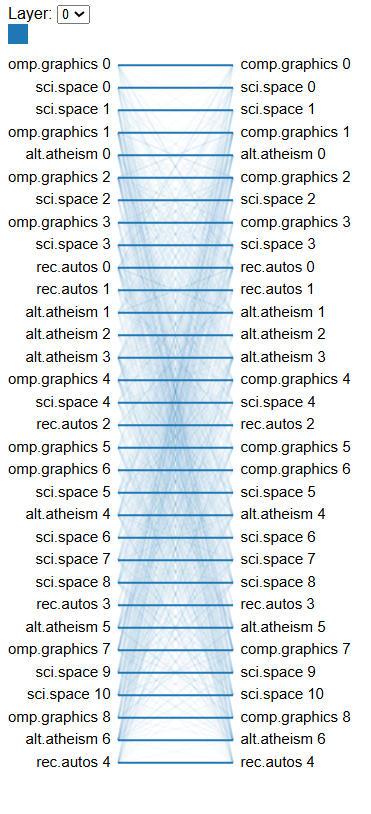
\includegraphics[width=0.45\textwidth]{../figures/4/attention_begin.png}
    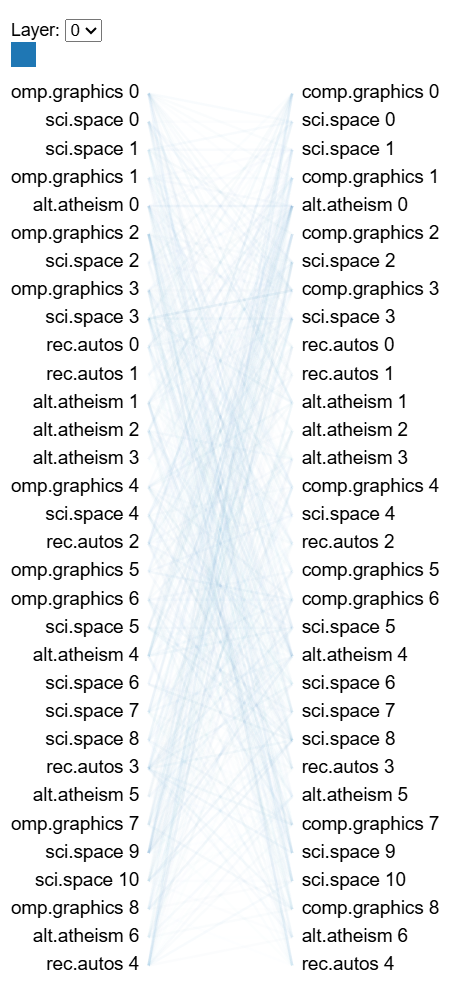
\includegraphics[width=0.45\textwidth]{../figures/4/attention_learned.png}
    \caption{Comparação entre a visualização de atenção inicial (TF-IDF) e após o treinamento (atenção aprendida)}
    \label{fig:attention_comparison}
\end{figure}